\documentclass[amsmath,amssymb,notitlepage,12pt]{revtex4}
%\documentclass[12pt]{article}
\usepackage[toc,page]{appendix}
\usepackage{graphicx}
\usepackage{bm}% bold math
\usepackage{multirow}
\usepackage{booktabs}
\usepackage{verbatim}
\usepackage{hyperref}
\usepackage{enumitem}
\hypersetup{pdftex,colorlinks=true,allcolors=blue}
\usepackage{hypcap}
\usepackage[small,compact]{titlesec}
\setlist[enumerate]{itemsep=0mm}
%\addtolength{\textwidth}{1cm}
%\addtolength{\hoffset}{-0.5cm}
\addtolength{\textheight}{1.2cm}
\addtolength{\voffset}{-0.0cm}
\begin{document}
\title{CLAS12 M{\o}ller Operations Manual - v0.1}
\date{\today}
\author{N. Baltzell, S. Stepanyan}
\begin{abstract}
\end{abstract}

\maketitle
%\tableofcontents
%\newpage

\section{Introduction}
The CLAS12 M{\o}ller system measures the polarization of the electron beam delivered to Hall B, and this document details its operating procedures.  The user interface for shift workers is shown in Fig.~\ref{fig:unconfig} and provides direct access to all controls and feedback that the normal operator should need, and its operating procedures are described in Section~\ref{sec:user}.  Expert operations are described in Section~\ref{sec:expert}.

\begin{figure}[htbp]\centering
    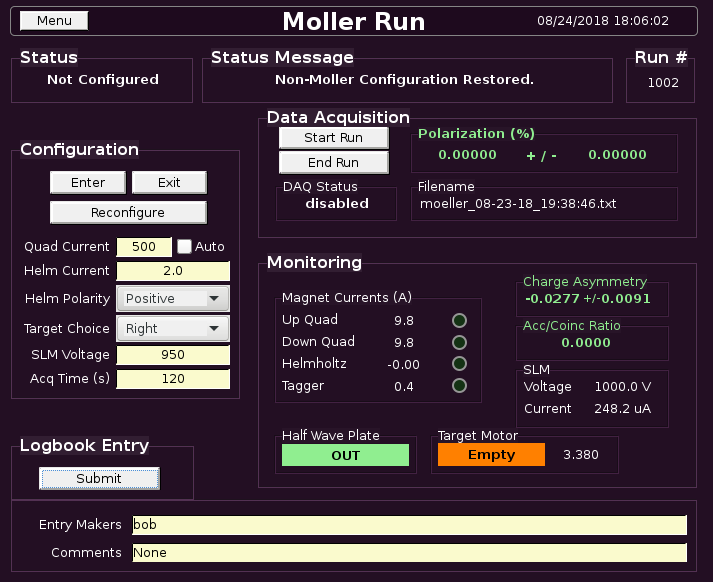
\includegraphics[width=11cm]{pics/unconfig}
    \caption{The user interface for shift workers for operating a M{\o}ller run is divided into status, configuration, data acquisition, monitoring, and logbook sections.  In this screenshot, the Moller symstem is not configured, i.e. the setup is for non-M{\o}ller beam delivery.\label{fig:unconfig}}
\end{figure}

\section{Standard Conditions}
The hardware settings are set automatically during the procedure in Section~\ref{sec:user}.  The quality requirements are to be monitored and maintained by the operator.

\subsection{Hadrware Settings}
The standard hardware settings for a M{\o}ller run are shown in Table~\ref{tab:pars}.  These are displayed in the Configuration section of Figure~\ref{fig:unconfig} and will be used to automatically configure all hardware during the procedure in the next section.

\begin{table}[htbp]\centering
    \begin{tabular}{ll}\toprule[1.5pt]
        SLM Voltage & 1400 V \\
        Collimator Position & Blank \\
        Target Position & Left \\
        Helmholtz Current & $\pm$3.5 A \\
        \cmidrule[0.5pt]{1-2}
        \multicolumn{2}{c}{Quadrupole Current} \\
        5-pass / 10.7 GeV & 3050 A\\
        3-pass / 6.4 GeV & 1350 A\\
        \bottomrule[1.5pt]
    \end{tabular}
    \caption{Standard hardware parameter values for the M{\o}ller setup.  Live values are shown in the Monitoring section in Figure~\ref{fig:unconfig}.\label{tab:pars}.}
\end{table}

\subsection{Quality Requirements}\label{sec:quality}
The requirements to be maintained during a M{\o}ller run, and the resulting desired error on the polarization measurement are shown in Table~\ref{tab:reqs}.
\begin{table}[htbp]\centering
    \begin{tabular}{ll}\toprule[1.5pt]
        2C21 BPM Current & $\sim$4 nA\\
        Beam Charge Asymmetry & $<0.1\%$\\
        Accidental/Coincidence Ratio & $<0.05$ \\
        Final Beam Polarization Error & $<2\%$ (absolute)\\
        \bottomrule[1.5pt]
    \end{tabular}
    \caption{Standard quality conditions required for a M{\o}ller run.  Live values are shown in the Monitoring and DAQ sections in Figure~\ref{fig:unconfig}.\label{tab:reqs}}
\end{table}
\section{Standard Procedures}\label{sec:user}
The procedure for the operator with the interface in Figure~\ref{fig:unconfig} can be summarized in the following steps, and more details are shown on the next page.
\begin{enumerate}
\vspace{-4mm}\item {\bf Configure}:  ensure the Configuration section is set as desired
\vspace{-4mm}\item {\bf Enter}: click {\em Enter} in the Configuration section and wait for success status
\vspace{-4mm}\item {\bf Start Run}: click {\em Start Run} in the DAQ section
\vspace{-4mm}\item {\bf Monitor}: monitor the critical parameters
\vspace{-4mm}\item {\bf End Run}: click {\em End Run} in the DAQ section
\vspace{-4mm}\item {\bf Log Entry}: click {\em Submit} in the Logbook Entry section 
\vspace{-4mm}\item {\bf Exit}: click {\em Exit} in the Configuration section and wait for success status
\end{enumerate}

\begin{enumerate}
\item {\bf Configure}:  ensure the Configuration section is set as desired
        \subitem
        The operator should confirm the desired values in Table~\ref{tab:pars} with the Configuration section of Figure~\ref{fig:unconfig}.  If the {\em Auto} option is selected for the quadrupoles, their current will be chosen based on standard settings for the current beam energy.  {\em Note, it is critical that some of these settings are held fixed while a run is ongoing, and those cannot be changed during a run from this interface.  See below regarding reconfiguring.}
\item {\bf Enter}: click {\em Enter} in the Configuration section and wait for success status
    \subitem Clicking the {\em Enter} button will configure the system for a M{\o}ller run by initiating a sequence of actions and provide corresponding feedback in the status portion of the screen.  This includes turning off some detectors' high voltage, inserting the blank collimator, energizing the quadrupoles and Helmholtz magnets, and inserting the M{\o}ller target.  Success will result in ``Moller Configuration Ready'' in the status message.
\item {\bf Start}: click {\em Start Run} in the DAQ section
    \subitem This will initiate a new M{\o}ller run, including zeroing any accumulated data, opening a new data file, incrementing the run number, and starting recording data.
\item {\bf Monitor}: monitor the critical parameters
    \subitem This is left to the operator and described in Section~\ref{sec:quality}.
\item {\bf End}: click {\em End Run} in the DAQ section
    \subitem At this point you should have achieved the desired polarization error of $2\%$, or just need to stop the current run and start a new one.
\item {\bf Log}: click {\em Submit} in the Logbook Entry section if the run was successful. 
    \subitem This will submit a log entry to HBLOG with a table summarizing the results and an attached data file. {\em Note, at this point you may navigate to the log entry in a web browser and add any relevant screenshots as comments to the entry}.
\item {\bf Rerun}  At this point you may reconfigure the system (e.g. change the Helmholtz polarity and click {\em Reconfigure}) and then start a second run, or just start another run with the same configuration.
\item {\bf Exit}: click {\em Exit} in the Configuration section and wait for success status
    \subitem  This will restore the non-M{\o}ller configuration by turning of the quadrupoles and Helmholtz and retracting the M{\o}ller target.  {\em Note, this will not restore any detector high voltage (except the SLM) nor move the collimator}. 
\end{enumerate}

\subsection{Status Values}
Describe the possible values of the status variable in the top left of the screen.

\section{Expert Procedures}\label{sec:expert}
The instructions for the old, manual procedure.

\subsection{Tuning Parameters}
\subsubsection{Injector}
\subsubsection{Quadrupoles}
\subsubsection{Beam Current}
\subsubsection{SLM Voltage}

\begin{appendices}
Description of the hardware and software involved in the CLAS12 M{\o}ller system.
\subsection{Quadrupoles}
\subsection{Helmholtz}
\subsection{Synchrotron Light Monitor}
\subsection{Target}
\subsection{Helicity Signal}
\subsection{Multi-Channel Scaler}
\subsection{EPICS IOCs}
\end{appendices}

\end{document}

